\section{Hardware Design}\label{sec:hw}
This section introduces the CNN accelerator we adopt in this work. We first introduce the architecture and energy model, and then the optimization to reduce the RRAM buffer dynamic energy cost.

\subsection{Architecture}\label{sec:hw:arch}

\begin{figure}[t]
  \centering
  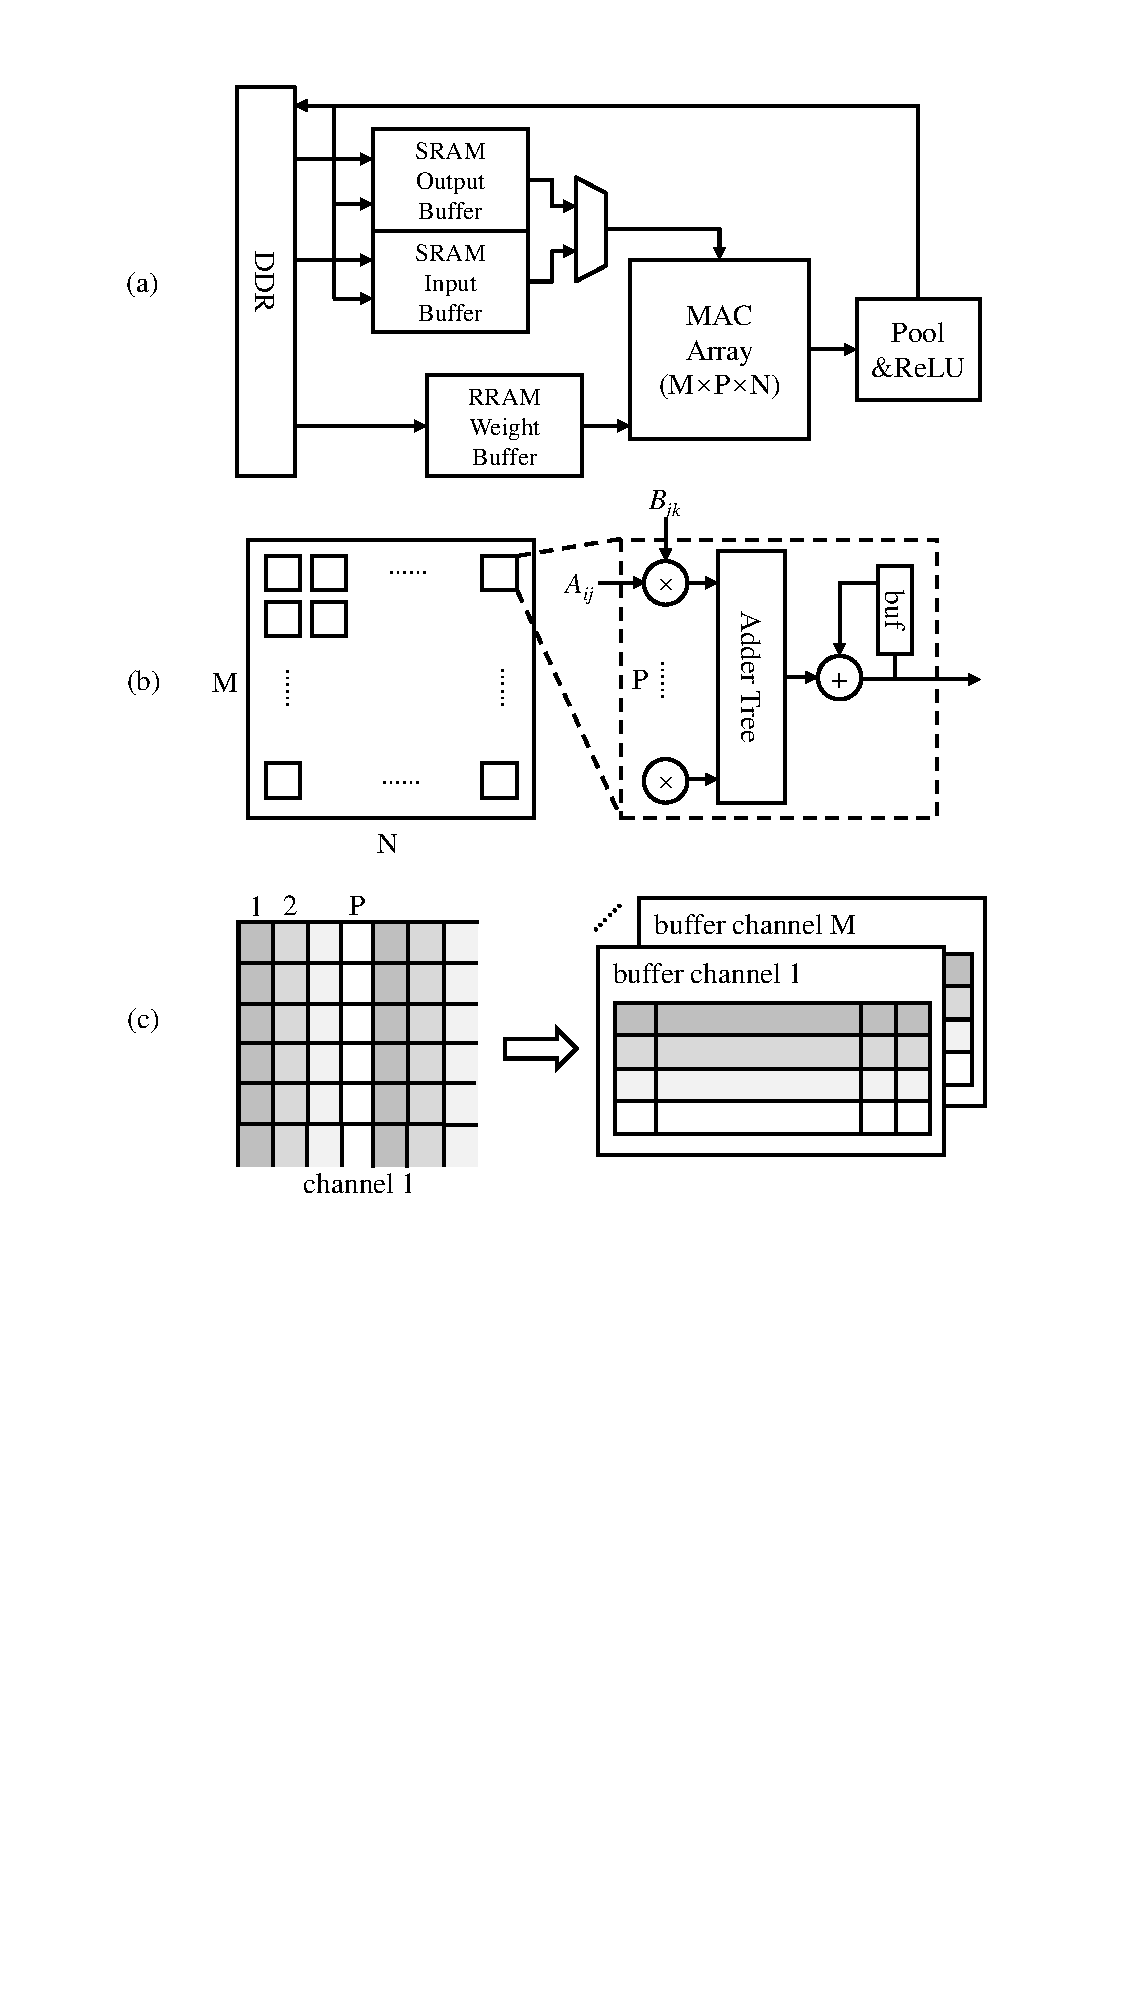
\includegraphics[width=1\columnwidth]{fig/arch.pdf}
  \vspace{-10pt}
  \caption{The CNN accelerator architecture. (a) The architecture mainly consists of a MAC array for computation and two levels of memory with on-chip buffers and external DDR. (b) MAC array structure for an $A_{p\times m}\times B_{m\times n}$ matrix-matrix multiplication. (c) Feature map buffer organization for sliding window data selection.}
  \vspace{-15pt}
  \label{fig:arch}
\end{figure}

The overall architecture is shown in Figure~\ref{fig:arch}(a). The system adopts DDR as external memory to support enough memory space. The on-chip memory consists of two buffers: input/output buffer and weight buffer. Input and output buffer stores feature maps during the process of a CNN. As the output of one layer serves as the input of the next, the input data of MAC array can be chosen from both of the buffers by a MUX unit. All the buffers work in a double-buffer way to cover the off-chip data transfer time with calculation time.

We first show how the process of CNN is parallelized with this design. As introduced in Section II A, a CNN layer consists of 4 nested loops. In this case, we unroll the feature map pixel loop, input channel loop and output channel loop as a $A_{m\times p}\times B_{p\times n}$ matrix-matrix multiplication. Each row of matrix A denotes the $p$ pixels read from a feature map and each $B_{ij}$ denotes a pixel in the convolution kernel corresponds to input channel $i$ and output $j$. Thus the convolution of $p$ pixels with $K\times K$ convolution kernels will be done with $\lceil M/m\rceil*K^2$ steps. The structure of the computation core is shown in Figure~\ref{fig:arch}(b). The array consists of $p\times n$ processing elements (PEs). Each of the PE implements a size-$m$ vector inner product in a pipelined manner. Each PE has an accumulator for its result. 

To support the above parallelization, a window selection function is needed for each channel stored in input/output buffer. In this design, we adopt the data mapping format as shown in Figure~\ref{fig:arch}(c). The pixels of each channel are stored in $p$ independent RAMs so that a size-$p$ window at any position can be selected from the buffer within a single cycle. Weight buffer can be implemented with a normal simple dual port RAM.

Consider the data access pattern, implement input/output buffers with RRAM is not practical. First, they require high write bandwidth to receive computation results from fast on-chip logic. Second, they require a high random access bandwidth, not sequential access bandwidth. Compared with input/output buffer, weight buffer only requires a high sequential access bandwidth. So in this work, we only consider implementing weight buffer with RRAM.


\subsection{Choosing the Loop Order}
With the parallelization strategy decided as introduced in section~\ref{sec:hw:arch}, the behavior of data access is affected by the order of the loops in the whole process. If we do not consider data transfer with DDR, the on-chip buffer energy cost comes from three aspects: input/output buffer read, weight buffer read, and input/output buffer write. To minimize this energy cost, we consider two loop execution order: kerel first and pixel first.

Kernel first order computes the $K\times K$ convolution on the $p$ pixels with $K^2$ cycles first, then move on to the next $p$ pixels. With this order, during the $K^2$ cycles, as the feature map window slides, the spatial locality of 2-d convoution is explored. Each feature map pixel is accessed only once. Pixel first order reuse the same weight in a $K\times K$ kernel and computes multiple $p$-pixel groups, then move on to the next weight. With this order, more feature map access is needed and intermediate result for each pixel group should be stored. This is not commonly adopted because intermediate result requires more bits for fixed-point data process. Suppose $c$ pixel groups are processed together, we compare the data access in Table~\ref{tab:ram_acc}. 

% Table generated by Excel2LaTeX from sheet 'Sheet1'
\begin{table}[htbp]
    \centering
    \caption{Data access comparison between kernel first order and pixel first order to calculate $c$ groups of $p$ pixels with $K\times K$ convolution.}
    \vspace{-5pt}
      \begin{tabular}{|r|r|r|}
      \hline
            & Kernel First & Pixel First \\
      \hline
      Input Feature Map & $cK(p+K-1)$ & $cpK^2$ \\
      \hline
      Weight & $cK^2$ & $K^2$ \\
      \hline
      Output Feature Map Rd & 0 & $cp(K^2-1)$ \\
      \hline
      Output Feature Map Wr & $cp$ & $cp(K^2-1)$ \\
      \hline
      \end{tabular}
    \label{tab:ram_acc}
  \end{table}

Directly using input/output buffer to store the intermediate result is not feasible because the intermediate result for fixed-point multiplication requires more bits. As RRAM has high read/write dynamic, we should try to reuse the weight to reduce access to weight buffer. In this design, we use a local accumulation buffer of size $2n$ as show in Figure~\ref{fig:arch}(b) to enable $n$ pixel groups processed together before written back to input/output buffer. This introduce extra on-chip memory cost. We examine the area and energy overhead in our experiment.